\documentclass[twoside]{book}

% Packages required by doxygen
\usepackage{fixltx2e}
\usepackage{calc}
\usepackage{doxygen}
\usepackage[export]{adjustbox} % also loads graphicx
\usepackage{graphicx}
\usepackage[utf8]{inputenc}
\usepackage{makeidx}
\usepackage{multicol}
\usepackage{multirow}
\PassOptionsToPackage{warn}{textcomp}
\usepackage{textcomp}
\usepackage[nointegrals]{wasysym}
\usepackage[table]{xcolor}

% Font selection
\usepackage[T1]{fontenc}
\usepackage[scaled=.90]{helvet}
\usepackage{courier}
\usepackage{amssymb}
\usepackage{sectsty}
\renewcommand{\familydefault}{\sfdefault}
\allsectionsfont{%
  \fontseries{bc}\selectfont%
  \color{darkgray}%
}
\renewcommand{\DoxyLabelFont}{%
  \fontseries{bc}\selectfont%
  \color{darkgray}%
}
\newcommand{\+}{\discretionary{\mbox{\scriptsize$\hookleftarrow$}}{}{}}

% Page & text layout
\usepackage{geometry}
\geometry{%
  a4paper,%
  top=2.5cm,%
  bottom=2.5cm,%
  left=2.5cm,%
  right=2.5cm%
}
\tolerance=750
\hfuzz=15pt
\hbadness=750
\setlength{\emergencystretch}{15pt}
\setlength{\parindent}{0cm}
\setlength{\parskip}{3ex plus 2ex minus 2ex}
\makeatletter
\renewcommand{\paragraph}{%
  \@startsection{paragraph}{4}{0ex}{-1.0ex}{1.0ex}{%
    \normalfont\normalsize\bfseries\SS@parafont%
  }%
}
\renewcommand{\subparagraph}{%
  \@startsection{subparagraph}{5}{0ex}{-1.0ex}{1.0ex}{%
    \normalfont\normalsize\bfseries\SS@subparafont%
  }%
}
\makeatother

% Headers & footers
\usepackage{fancyhdr}
\pagestyle{fancyplain}
\fancyhead[LE]{\fancyplain{}{\bfseries\thepage}}
\fancyhead[CE]{\fancyplain{}{}}
\fancyhead[RE]{\fancyplain{}{\bfseries\leftmark}}
\fancyhead[LO]{\fancyplain{}{\bfseries\rightmark}}
\fancyhead[CO]{\fancyplain{}{}}
\fancyhead[RO]{\fancyplain{}{\bfseries\thepage}}
\fancyfoot[LE]{\fancyplain{}{}}
\fancyfoot[CE]{\fancyplain{}{}}
\fancyfoot[RE]{\fancyplain{}{\bfseries\scriptsize Generated by Doxygen }}
\fancyfoot[LO]{\fancyplain{}{\bfseries\scriptsize Generated by Doxygen }}
\fancyfoot[CO]{\fancyplain{}{}}
\fancyfoot[RO]{\fancyplain{}{}}
\renewcommand{\footrulewidth}{0.4pt}
\renewcommand{\chaptermark}[1]{%
  \markboth{#1}{}%
}
\renewcommand{\sectionmark}[1]{%
  \markright{\thesection\ #1}%
}

% Indices & bibliography
\usepackage{natbib}
\usepackage[titles]{tocloft}
\setcounter{tocdepth}{3}
\setcounter{secnumdepth}{5}
\makeindex

% Hyperlinks (required, but should be loaded last)
\usepackage{ifpdf}
\ifpdf
  \usepackage[pdftex,pagebackref=true]{hyperref}
\else
  \usepackage[ps2pdf,pagebackref=true]{hyperref}
\fi
\hypersetup{%
  colorlinks=true,%
  linkcolor=blue,%
  citecolor=blue,%
  unicode%
}

% Custom commands
\newcommand{\clearemptydoublepage}{%
  \newpage{\pagestyle{empty}\cleardoublepage}%
}

\usepackage{caption}
\captionsetup{labelsep=space,justification=centering,font={bf},singlelinecheck=off,skip=4pt,position=top}

%===== C O N T E N T S =====

\begin{document}

% Titlepage & ToC
\hypersetup{pageanchor=false,
             bookmarksnumbered=true,
             pdfencoding=unicode
            }
\pagenumbering{alph}
\begin{titlepage}
\vspace*{7cm}
\begin{center}%
{\Large Engine }\\
\vspace*{1cm}
{\large Generated by Doxygen 1.8.14}\\
\end{center}
\end{titlepage}
\clearemptydoublepage
\pagenumbering{roman}
\tableofcontents
\clearemptydoublepage
\pagenumbering{arabic}
\hypersetup{pageanchor=true}

%--- Begin generated contents ---
\chapter{Engine}
\label{md__home_adam_Desktop_Engine_README}
\Hypertarget{md__home_adam_Desktop_Engine_README}
Physics and Rendering Engine 
\chapter{Hierarchical Index}
\section{Class Hierarchy}
This inheritance list is sorted roughly, but not completely, alphabetically\+:\begin{DoxyCompactList}
\item \contentsline{section}{Camera}{\pageref{classCamera}}{}
\item \contentsline{section}{Force\+Generator}{\pageref{classForceGenerator}}{}
\begin{DoxyCompactList}
\item \contentsline{section}{Constant\+Force\+Generator}{\pageref{classConstantForceGenerator}}{}
\end{DoxyCompactList}
\item \contentsline{section}{Mesh}{\pageref{classMesh}}{}
\item \contentsline{section}{Model}{\pageref{classModel}}{}
\begin{DoxyCompactList}
\item \contentsline{section}{Sphere}{\pageref{classSphere}}{}
\end{DoxyCompactList}
\item \contentsline{section}{Physics\+Entity}{\pageref{classPhysicsEntity}}{}
\begin{DoxyCompactList}
\item \contentsline{section}{Sphere}{\pageref{classSphere}}{}
\end{DoxyCompactList}
\item \contentsline{section}{Scene}{\pageref{classScene}}{}
\item \contentsline{section}{Shader}{\pageref{classShader}}{}
\item \contentsline{section}{Time\+Integrator}{\pageref{classTimeIntegrator}}{}
\begin{DoxyCompactList}
\item \contentsline{section}{Explicit\+Euler}{\pageref{classExplicitEuler}}{}
\end{DoxyCompactList}
\end{DoxyCompactList}

\chapter{Class Index}
\section{Class List}
Here are the classes, structs, unions and interfaces with brief descriptions\+:\begin{DoxyCompactList}
\item\contentsline{section}{\hyperlink{classCamera}{Camera} \\*A \hyperlink{classCamera}{Camera} is used to view a scene from a particular vantage point }{\pageref{classCamera}}{}
\item\contentsline{section}{\hyperlink{classConstantForceGenerator}{Constant\+Force\+Generator} \\*A constant force throughout all space }{\pageref{classConstantForceGenerator}}{}
\item\contentsline{section}{\hyperlink{classExplicitEuler}{Explicit\+Euler} \\*Implementation of Explicit Euler method for solving Newton\textquotesingle{}s equations of motion }{\pageref{classExplicitEuler}}{}
\item\contentsline{section}{\hyperlink{classForceGenerator}{Force\+Generator} \\*Abstract base class for all force generators }{\pageref{classForceGenerator}}{}
\item\contentsline{section}{\hyperlink{classMesh}{Mesh} \\*Defines a mesh }{\pageref{classMesh}}{}
\item\contentsline{section}{\hyperlink{classModel}{Model} \\*Defines a model used for rendering }{\pageref{classModel}}{}
\item\contentsline{section}{\hyperlink{classPhysicsEntity}{Physics\+Entity} \\*An entity subject to the laws of physics }{\pageref{classPhysicsEntity}}{}
\item\contentsline{section}{\hyperlink{classScene}{Scene} \\*A scene in the engine }{\pageref{classScene}}{}
\item\contentsline{section}{\hyperlink{classShader}{Shader} }{\pageref{classShader}}{}
\item\contentsline{section}{\hyperlink{classSphere}{Sphere} \\*A sphere }{\pageref{classSphere}}{}
\item\contentsline{section}{\hyperlink{classTimeIntegrator}{Time\+Integrator} \\*An abstact base class for all grid based numerical O\+DE solvers for Newton\textquotesingle{}s laws }{\pageref{classTimeIntegrator}}{}
\end{DoxyCompactList}

\chapter{Class Documentation}
\hypertarget{classCamera}{}\section{Camera Class Reference}
\label{classCamera}\index{Camera@{Camera}}
\subsection*{Public Member Functions}
\begin{DoxyCompactItemize}
\item 
\mbox{\Hypertarget{classCamera_a852d8c105b562be494204cac8518b66f}\label{classCamera_a852d8c105b562be494204cac8518b66f}} 
{\bfseries Camera} (Vector3\+Gf position=Vector3\+Gf(0.\+0f, 0.\+0f, 0.\+0f), Vector3\+Gf up=\+Vector3\+Gf(0.\+0f, 1.\+0f, 0.\+0f), G\+Lfloat yaw=\+Y\+A\+W, G\+Lfloat pitch=\+P\+I\+T\+C\+H)
\item 
\mbox{\Hypertarget{classCamera_a1efd973829c22d5fe15a26ede3357ee5}\label{classCamera_a1efd973829c22d5fe15a26ede3357ee5}} 
{\bfseries Camera} (G\+Lfloat posX, G\+Lfloat posY, G\+Lfloat posZ, G\+Lfloat upX, G\+Lfloat upY, G\+Lfloat upZ, G\+Lfloat yaw, G\+Lfloat pitch)
\item 
\mbox{\Hypertarget{classCamera_af040480b69b4235d9bd203bf6775e79a}\label{classCamera_af040480b69b4235d9bd203bf6775e79a}} 
Eigen\+::\+Matrix$<$ G\+Lfloat, 4, 4 $>$ {\bfseries Get\+View\+Matrix} ()
\item 
\mbox{\Hypertarget{classCamera_ac7e9a7f3e63c670fd695a8f03d02dbdf}\label{classCamera_ac7e9a7f3e63c670fd695a8f03d02dbdf}} 
void {\bfseries Process\+Keyboard} (Camera\+\_\+\+Movement direction, G\+Lfloat delta\+Time)
\item 
\mbox{\Hypertarget{classCamera_a97ffbf8d8935fc63bd2ca71a4268eec4}\label{classCamera_a97ffbf8d8935fc63bd2ca71a4268eec4}} 
void {\bfseries Process\+Mouse\+Movement} (G\+Lfloat xoffset, G\+Lfloat yoffset, G\+Lboolean constrain\+Pitch=true)
\item 
\mbox{\Hypertarget{classCamera_af269e5ef38e791afb7f4a1dfb8da2399}\label{classCamera_af269e5ef38e791afb7f4a1dfb8da2399}} 
void {\bfseries Process\+Mouse\+Scroll} (G\+Lfloat yoffset)
\end{DoxyCompactItemize}
\subsection*{Public Attributes}
\begin{DoxyCompactItemize}
\item 
\mbox{\Hypertarget{classCamera_ab24ae04e34fbcc1057be0ccca9ce5d76}\label{classCamera_ab24ae04e34fbcc1057be0ccca9ce5d76}} 
Vector3\+Gf {\bfseries Position}
\item 
\mbox{\Hypertarget{classCamera_a7ead2f5965525cc388b16baaf7730e2b}\label{classCamera_a7ead2f5965525cc388b16baaf7730e2b}} 
Vector3\+Gf {\bfseries Front}
\item 
\mbox{\Hypertarget{classCamera_a034f566309116c5e31bf31fc3ae668a5}\label{classCamera_a034f566309116c5e31bf31fc3ae668a5}} 
Vector3\+Gf {\bfseries Up}
\item 
\mbox{\Hypertarget{classCamera_ab720984bfc18071ec793fceb0174f6e5}\label{classCamera_ab720984bfc18071ec793fceb0174f6e5}} 
Vector3\+Gf {\bfseries Right}
\item 
\mbox{\Hypertarget{classCamera_a37ce2216fcfd5a5f58913ebd320981aa}\label{classCamera_a37ce2216fcfd5a5f58913ebd320981aa}} 
Vector3\+Gf {\bfseries World\+Up}
\item 
\mbox{\Hypertarget{classCamera_abf27283ca0ccc51bae8446796ffc6b44}\label{classCamera_abf27283ca0ccc51bae8446796ffc6b44}} 
G\+Lfloat {\bfseries Yaw}
\item 
\mbox{\Hypertarget{classCamera_ae6afc2507f67baf4390405cfda1d1e87}\label{classCamera_ae6afc2507f67baf4390405cfda1d1e87}} 
G\+Lfloat {\bfseries Pitch}
\item 
\mbox{\Hypertarget{classCamera_a93ea63669df9617a6f63fa09e74a01a9}\label{classCamera_a93ea63669df9617a6f63fa09e74a01a9}} 
G\+Lfloat {\bfseries Movement\+Speed}
\item 
\mbox{\Hypertarget{classCamera_adc61747052dc386a4ab8e110a1fbc628}\label{classCamera_adc61747052dc386a4ab8e110a1fbc628}} 
G\+Lfloat {\bfseries Mouse\+Sensitivity}
\item 
\mbox{\Hypertarget{classCamera_a1078d85d2e18bdc32291aabfcdda710a}\label{classCamera_a1078d85d2e18bdc32291aabfcdda710a}} 
G\+Lfloat {\bfseries Zoom}
\end{DoxyCompactItemize}


The documentation for this class was generated from the following file\+:\begin{DoxyCompactItemize}
\item 
/home/adam/\+Desktop/\+Engine/include/camera.\+h\end{DoxyCompactItemize}

\hypertarget{classConstantForceGenerator}{}\section{Constant\+Force\+Generator Class Reference}
\label{classConstantForceGenerator}\index{Constant\+Force\+Generator@{Constant\+Force\+Generator}}


A constant force throughout all space.  




{\ttfamily \#include $<$constant\+\_\+force.\+h$>$}

Inheritance diagram for Constant\+Force\+Generator\+:\begin{figure}[H]
\begin{center}
\leavevmode
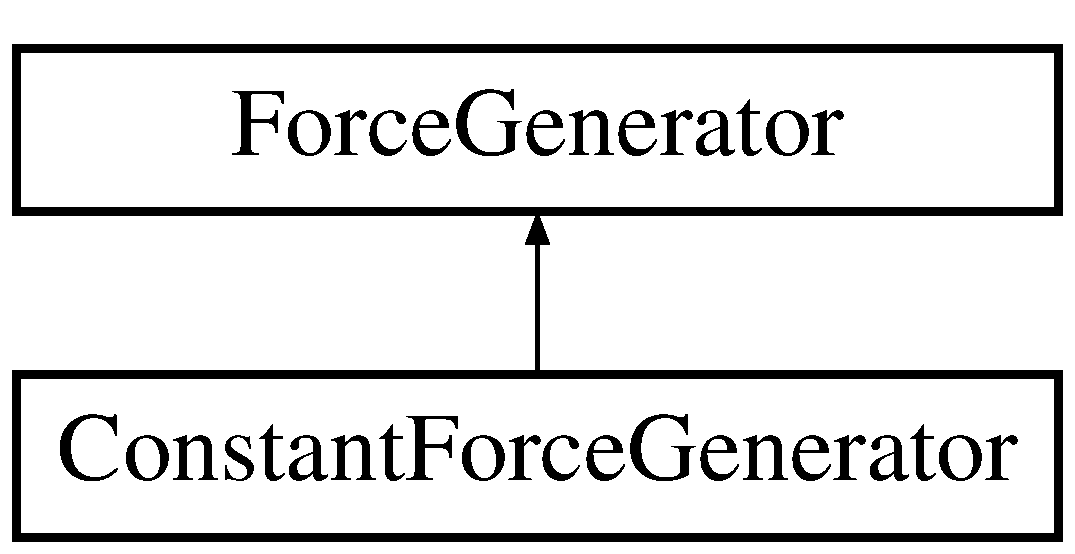
\includegraphics[height=2.000000cm]{classConstantForceGenerator}
\end{center}
\end{figure}
\subsection*{Public Member Functions}
\begin{DoxyCompactItemize}
\item 
\hyperlink{classConstantForceGenerator_a1313aa10929f00280d1f3d5e961f7352}{Constant\+Force\+Generator} ()
\item 
\hyperlink{classConstantForceGenerator_a6ff2c05d06addf1859a604c6dbb8f9bd}{Constant\+Force\+Generator} (Vector3\+Gf accel)
\item 
\hyperlink{classConstantForceGenerator_a3563efee2f73fd5c2e504db89b4d3767}{$\sim$\+Constant\+Force\+Generator} ()
\item 
void \hyperlink{classConstantForceGenerator_a6a50c67567de9d26073a373aed77d29f}{Accumulate\+Force} (std\+::shared\+\_\+ptr$<$ \hyperlink{classPhysicsEntity}{Physics\+Entity} $>$ entity, Vector3\+Gf \&F)
\end{DoxyCompactItemize}


\subsection{Detailed Description}
A constant force throughout all space. 

\subsection{Constructor \& Destructor Documentation}
\mbox{\Hypertarget{classConstantForceGenerator_a1313aa10929f00280d1f3d5e961f7352}\label{classConstantForceGenerator_a1313aa10929f00280d1f3d5e961f7352}} 
\index{Constant\+Force\+Generator@{Constant\+Force\+Generator}!Constant\+Force\+Generator@{Constant\+Force\+Generator}}
\index{Constant\+Force\+Generator@{Constant\+Force\+Generator}!Constant\+Force\+Generator@{Constant\+Force\+Generator}}
\subsubsection{\texorpdfstring{Constant\+Force\+Generator()}{ConstantForceGenerator()}\hspace{0.1cm}{\footnotesize\ttfamily [1/2]}}
{\footnotesize\ttfamily Constant\+Force\+Generator\+::\+Constant\+Force\+Generator (\begin{DoxyParamCaption}{ }\end{DoxyParamCaption})}

Builds a \hyperlink{classConstantForceGenerator}{Constant\+Force\+Generator} with a zero acceleration at all points in space. \mbox{\Hypertarget{classConstantForceGenerator_a6ff2c05d06addf1859a604c6dbb8f9bd}\label{classConstantForceGenerator_a6ff2c05d06addf1859a604c6dbb8f9bd}} 
\index{Constant\+Force\+Generator@{Constant\+Force\+Generator}!Constant\+Force\+Generator@{Constant\+Force\+Generator}}
\index{Constant\+Force\+Generator@{Constant\+Force\+Generator}!Constant\+Force\+Generator@{Constant\+Force\+Generator}}
\subsubsection{\texorpdfstring{Constant\+Force\+Generator()}{ConstantForceGenerator()}\hspace{0.1cm}{\footnotesize\ttfamily [2/2]}}
{\footnotesize\ttfamily Constant\+Force\+Generator\+::\+Constant\+Force\+Generator (\begin{DoxyParamCaption}\item[{Vector3\+Gf}]{accel }\end{DoxyParamCaption})}

Builds a \hyperlink{classConstantForceGenerator}{Constant\+Force\+Generator} with a given acceleration at all points in space 
\begin{DoxyParams}{Parameters}
{\em accel} & acceleration vector for the force \\
\hline
\end{DoxyParams}
\mbox{\Hypertarget{classConstantForceGenerator_a3563efee2f73fd5c2e504db89b4d3767}\label{classConstantForceGenerator_a3563efee2f73fd5c2e504db89b4d3767}} 
\index{Constant\+Force\+Generator@{Constant\+Force\+Generator}!````~Constant\+Force\+Generator@{$\sim$\+Constant\+Force\+Generator}}
\index{````~Constant\+Force\+Generator@{$\sim$\+Constant\+Force\+Generator}!Constant\+Force\+Generator@{Constant\+Force\+Generator}}
\subsubsection{\texorpdfstring{$\sim$\+Constant\+Force\+Generator()}{~ConstantForceGenerator()}}
{\footnotesize\ttfamily Constant\+Force\+Generator\+::$\sim$\+Constant\+Force\+Generator (\begin{DoxyParamCaption}{ }\end{DoxyParamCaption})}

Deconstructs a \hyperlink{classConstantForceGenerator}{Constant\+Force\+Generator} 

\subsection{Member Function Documentation}
\mbox{\Hypertarget{classConstantForceGenerator_a6a50c67567de9d26073a373aed77d29f}\label{classConstantForceGenerator_a6a50c67567de9d26073a373aed77d29f}} 
\index{Constant\+Force\+Generator@{Constant\+Force\+Generator}!Accumulate\+Force@{Accumulate\+Force}}
\index{Accumulate\+Force@{Accumulate\+Force}!Constant\+Force\+Generator@{Constant\+Force\+Generator}}
\subsubsection{\texorpdfstring{Accumulate\+Force()}{AccumulateForce()}}
{\footnotesize\ttfamily void Constant\+Force\+Generator\+::\+Accumulate\+Force (\begin{DoxyParamCaption}\item[{std\+::shared\+\_\+ptr$<$ \hyperlink{classPhysicsEntity}{Physics\+Entity} $>$}]{entity,  }\item[{Vector3\+Gf \&}]{F }\end{DoxyParamCaption})\hspace{0.3cm}{\ttfamily [virtual]}}

Adds a constant force determined by the mass of the provided entity and the stored acceleration vector 
\begin{DoxyParams}{Parameters}
{\em entity} & Entity whom the force will be applied against \\
\hline
{\em F} & Force vector that will accumulate the constant force represented by this instance \\
\hline
\end{DoxyParams}


Implements \hyperlink{classForceGenerator}{Force\+Generator}.



The documentation for this class was generated from the following files\+:\begin{DoxyCompactItemize}
\item 
/home/adam/\+Desktop/\+Engine/include/constant\+\_\+force.\+h\item 
/home/adam/\+Desktop/\+Engine/constant\+\_\+force.\+cpp\end{DoxyCompactItemize}

\hypertarget{classExplicitEuler}{}\section{Explicit\+Euler Class Reference}
\label{classExplicitEuler}\index{Explicit\+Euler@{Explicit\+Euler}}


Implementation of Explicit Euler method for solving Newton\textquotesingle{}s equations of motion.  




{\ttfamily \#include $<$explicit\+\_\+euler.\+h$>$}

Inheritance diagram for Explicit\+Euler\+:\begin{figure}[H]
\begin{center}
\leavevmode
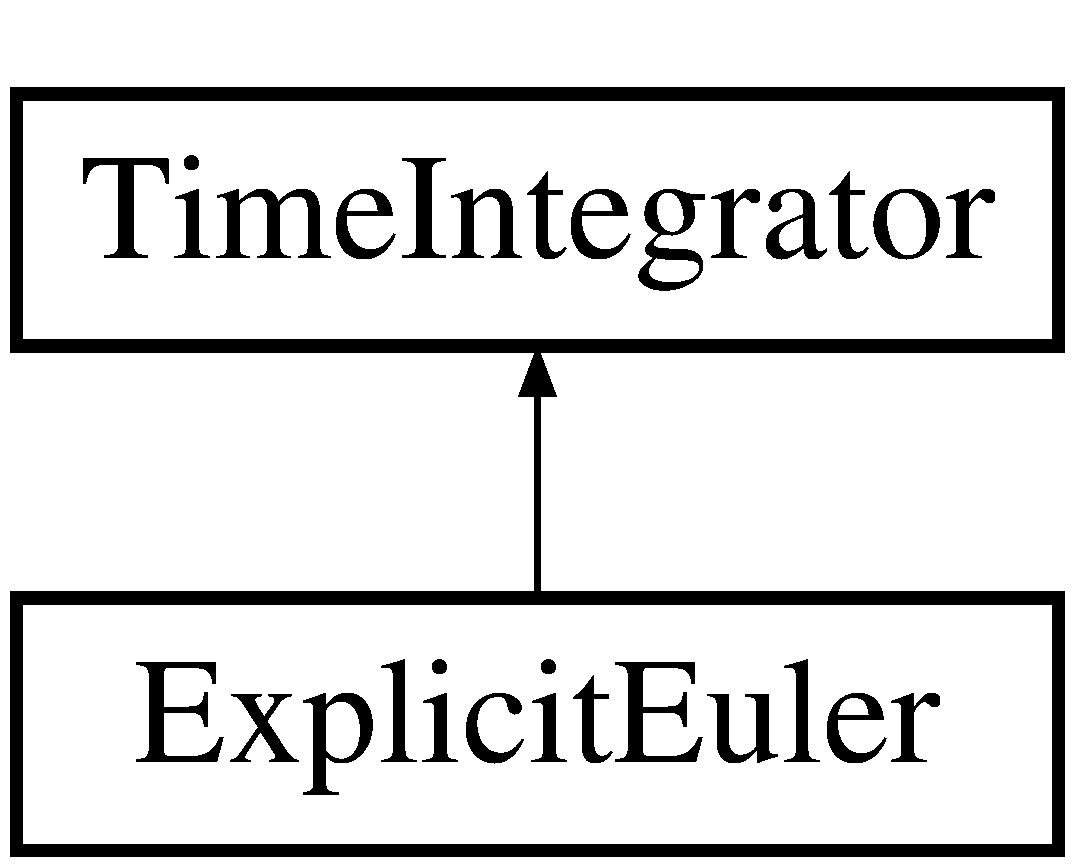
\includegraphics[height=2.000000cm]{classExplicitEuler}
\end{center}
\end{figure}
\subsection*{Public Member Functions}
\begin{DoxyCompactItemize}
\item 
\hyperlink{classExplicitEuler_aa16df6a77bb175fdd6291c302cb61d17}{Explicit\+Euler} ()
\item 
\hyperlink{classExplicitEuler_ab7ba8cf17d34831178c47a3a3711c3b0}{Explicit\+Euler} (G\+Lfloat dt)
\item 
void \hyperlink{classExplicitEuler_aee3f98264fab0eac7517d9dc8487ecb4}{Solve} (const Vector3\+Gf xi, const Vector3\+Gf vi, const G\+Lfloat mass, const Vector3\+Gf F, Vector3\+Gf \&xf, Vector3\+Gf \&vf)
\end{DoxyCompactItemize}
\subsection*{Additional Inherited Members}


\subsection{Detailed Description}
Implementation of Explicit Euler method for solving Newton\textquotesingle{}s equations of motion. 

\subsection{Constructor \& Destructor Documentation}
\mbox{\Hypertarget{classExplicitEuler_aa16df6a77bb175fdd6291c302cb61d17}\label{classExplicitEuler_aa16df6a77bb175fdd6291c302cb61d17}} 
\index{Explicit\+Euler@{Explicit\+Euler}!Explicit\+Euler@{Explicit\+Euler}}
\index{Explicit\+Euler@{Explicit\+Euler}!Explicit\+Euler@{Explicit\+Euler}}
\subsubsection{\texorpdfstring{Explicit\+Euler()}{ExplicitEuler()}\hspace{0.1cm}{\footnotesize\ttfamily [1/2]}}
{\footnotesize\ttfamily Explicit\+Euler\+::\+Explicit\+Euler (\begin{DoxyParamCaption}{ }\end{DoxyParamCaption})}

Constructs an instance of Exlplict\+Euler with a default grid size \mbox{\Hypertarget{classExplicitEuler_ab7ba8cf17d34831178c47a3a3711c3b0}\label{classExplicitEuler_ab7ba8cf17d34831178c47a3a3711c3b0}} 
\index{Explicit\+Euler@{Explicit\+Euler}!Explicit\+Euler@{Explicit\+Euler}}
\index{Explicit\+Euler@{Explicit\+Euler}!Explicit\+Euler@{Explicit\+Euler}}
\subsubsection{\texorpdfstring{Explicit\+Euler()}{ExplicitEuler()}\hspace{0.1cm}{\footnotesize\ttfamily [2/2]}}
{\footnotesize\ttfamily Explicit\+Euler\+::\+Explicit\+Euler (\begin{DoxyParamCaption}\item[{G\+Lfloat}]{dt }\end{DoxyParamCaption})}

Constructs an instance of \hyperlink{classExplicitEuler}{Explicit\+Euler} with the provided grid size 
\begin{DoxyParams}{Parameters}
{\em dt} & difference between two points on the grid \\
\hline
\end{DoxyParams}


\subsection{Member Function Documentation}
\mbox{\Hypertarget{classExplicitEuler_aee3f98264fab0eac7517d9dc8487ecb4}\label{classExplicitEuler_aee3f98264fab0eac7517d9dc8487ecb4}} 
\index{Explicit\+Euler@{Explicit\+Euler}!Solve@{Solve}}
\index{Solve@{Solve}!Explicit\+Euler@{Explicit\+Euler}}
\subsubsection{\texorpdfstring{Solve()}{Solve()}}
{\footnotesize\ttfamily void Explicit\+Euler\+::\+Solve (\begin{DoxyParamCaption}\item[{const Vector3\+Gf}]{xi,  }\item[{const Vector3\+Gf}]{vi,  }\item[{const G\+Lfloat}]{mass,  }\item[{const Vector3\+Gf}]{F,  }\item[{Vector3\+Gf \&}]{xf,  }\item[{Vector3\+Gf \&}]{vf }\end{DoxyParamCaption})\hspace{0.3cm}{\ttfamily [virtual]}}

Solves Newton\textquotesingle{}s equations of motion 
\begin{DoxyParams}{Parameters}
{\em xi} & intial position of entity \\
\hline
{\em vi} & initial velocity of entity \\
\hline
{\em mass} & mass of entity \\
\hline
{\em xf} & Final poisition of entity. This will be updated with the new position for the next grid point \\
\hline
{\em vf} & Final velocity of entity. This will be ipdated with the new velocity for the next grid point \\
\hline
\end{DoxyParams}


Implements \hyperlink{classTimeIntegrator}{Time\+Integrator}.



The documentation for this class was generated from the following files\+:\begin{DoxyCompactItemize}
\item 
/home/adam/\+Desktop/\+Engine/include/explicit\+\_\+euler.\+h\item 
/home/adam/\+Desktop/\+Engine/explicit\+\_\+euler.\+cpp\end{DoxyCompactItemize}

\hypertarget{classForceGenerator}{}\section{Force\+Generator Class Reference}
\label{classForceGenerator}\index{Force\+Generator@{Force\+Generator}}
Inheritance diagram for Force\+Generator\+:\begin{figure}[H]
\begin{center}
\leavevmode
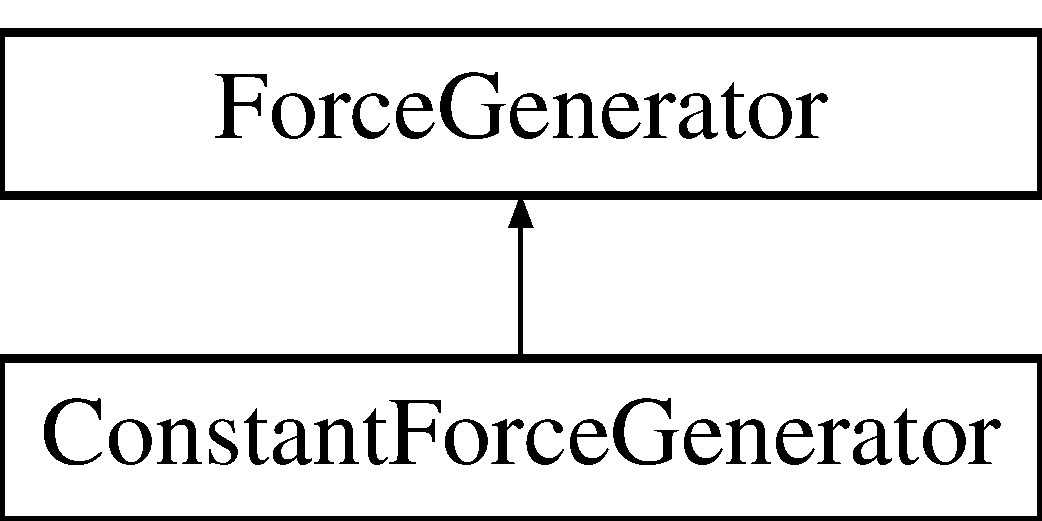
\includegraphics[height=2.000000cm]{classForceGenerator}
\end{center}
\end{figure}
\subsection*{Public Member Functions}
\begin{DoxyCompactItemize}
\item 
\mbox{\Hypertarget{classForceGenerator_a96cae0febb1fa8a0bb017aba7b82dbe8}\label{classForceGenerator_a96cae0febb1fa8a0bb017aba7b82dbe8}} 
virtual void {\bfseries Accumulate\+Force} (std\+::shared\+\_\+ptr$<$ \hyperlink{classPhysicsEntity}{Physics\+Entity} $>$ entity, Vector3\+Gf \&F)=0
\end{DoxyCompactItemize}


The documentation for this class was generated from the following file\+:\begin{DoxyCompactItemize}
\item 
/home/adam/\+Desktop/\+Engine/include/force\+\_\+generator.\+h\end{DoxyCompactItemize}

\hypertarget{classMesh}{}\section{Mesh Class Reference}
\label{classMesh}\index{Mesh@{Mesh}}


Defines a mesh.  




{\ttfamily \#include $<$mesh.\+h$>$}

\subsection*{Public Member Functions}
\begin{DoxyCompactItemize}
\item 
\hyperlink{classMesh_a2af137f1571af89172b9c102302c416b}{Mesh} ()
\item 
\hyperlink{classMesh_acca57d57a35d834a9ba0fa0290a4d121}{Mesh} (std\+::vector$<$ G\+Lfloat $>$ vertices, std\+::vector$<$ std\+::pair$<$ G\+Luint, G\+Luint $>$$>$ edges)
\item 
std\+::vector$<$ G\+Lfloat $>$ \hyperlink{classMesh_aad4e49df1b12331d688d677f997360a5}{Get\+Vertices} ()
\item 
std\+::vector$<$ std\+::pair$<$ G\+Luint, G\+Luint $>$ $>$ \hyperlink{classMesh_a4c31bac7ef0c5552e8dc692a33726ca3}{Get\+Edges} ()
\item 
G\+Luint \hyperlink{classMesh_adbbf05c59fd7cc170ceca2a0a71d7af1}{Get\+Num\+Edges} ()
\item 
G\+Luint \hyperlink{classMesh_ad4917bc56c71f31974af4be3eb90a390}{Get\+V\+AO} ()
\item 
void \hyperlink{classMesh_abe1f7ce31904fb28cef0c156b892af8e}{Clean\+Up} ()
\end{DoxyCompactItemize}


\subsection{Detailed Description}
Defines a mesh. 

A mesh is represented by a list of vertices and edges. A vertex is a set of 3 floats representing a (x,y,z) pair in R$^\wedge$3. An Edge is represented by a pair of indices into the vertex list. Vertices in edges are listed in clockwise order as they appear on the mesh. Once a mesh is built it is loaded onto the G\+PU so it can be rendered 

\subsection{Constructor \& Destructor Documentation}
\mbox{\Hypertarget{classMesh_a2af137f1571af89172b9c102302c416b}\label{classMesh_a2af137f1571af89172b9c102302c416b}} 
\index{Mesh@{Mesh}!Mesh@{Mesh}}
\index{Mesh@{Mesh}!Mesh@{Mesh}}
\subsubsection{\texorpdfstring{Mesh()}{Mesh()}\hspace{0.1cm}{\footnotesize\ttfamily [1/2]}}
{\footnotesize\ttfamily Mesh\+::\+Mesh (\begin{DoxyParamCaption}{ }\end{DoxyParamCaption})}

Builds a mesh with no vertices or edges \mbox{\Hypertarget{classMesh_acca57d57a35d834a9ba0fa0290a4d121}\label{classMesh_acca57d57a35d834a9ba0fa0290a4d121}} 
\index{Mesh@{Mesh}!Mesh@{Mesh}}
\index{Mesh@{Mesh}!Mesh@{Mesh}}
\subsubsection{\texorpdfstring{Mesh()}{Mesh()}\hspace{0.1cm}{\footnotesize\ttfamily [2/2]}}
{\footnotesize\ttfamily Mesh\+::\+Mesh (\begin{DoxyParamCaption}\item[{std\+::vector$<$ G\+Lfloat $>$}]{vertices,  }\item[{std\+::vector$<$ std\+::pair$<$ G\+Luint, G\+Luint $>$$>$}]{edges }\end{DoxyParamCaption})}

Builds a mesh with the provided vertices and edges 
\begin{DoxyParams}{Parameters}
{\em vertices} & List of vertices for the mesh. It\textquotesingle{}s length should be a multiple of 3 \\
\hline
{\em edges} & List of edges for the mesh. Listed in clockwise order \\
\hline
\end{DoxyParams}


\subsection{Member Function Documentation}
\mbox{\Hypertarget{classMesh_abe1f7ce31904fb28cef0c156b892af8e}\label{classMesh_abe1f7ce31904fb28cef0c156b892af8e}} 
\index{Mesh@{Mesh}!Clean\+Up@{Clean\+Up}}
\index{Clean\+Up@{Clean\+Up}!Mesh@{Mesh}}
\subsubsection{\texorpdfstring{Clean\+Up()}{CleanUp()}}
{\footnotesize\ttfamily void Mesh\+::\+Clean\+Up (\begin{DoxyParamCaption}{ }\end{DoxyParamCaption})}

Removes the mesh from the G\+PU \mbox{\Hypertarget{classMesh_a4c31bac7ef0c5552e8dc692a33726ca3}\label{classMesh_a4c31bac7ef0c5552e8dc692a33726ca3}} 
\index{Mesh@{Mesh}!Get\+Edges@{Get\+Edges}}
\index{Get\+Edges@{Get\+Edges}!Mesh@{Mesh}}
\subsubsection{\texorpdfstring{Get\+Edges()}{GetEdges()}}
{\footnotesize\ttfamily std\+::vector$<$ std\+::pair$<$ G\+Luint, G\+Luint $>$ $>$ Mesh\+::\+Get\+Edges (\begin{DoxyParamCaption}{ }\end{DoxyParamCaption})}

\begin{DoxyReturn}{Returns}
A copy of the edges in the mesh 
\end{DoxyReturn}
\mbox{\Hypertarget{classMesh_adbbf05c59fd7cc170ceca2a0a71d7af1}\label{classMesh_adbbf05c59fd7cc170ceca2a0a71d7af1}} 
\index{Mesh@{Mesh}!Get\+Num\+Edges@{Get\+Num\+Edges}}
\index{Get\+Num\+Edges@{Get\+Num\+Edges}!Mesh@{Mesh}}
\subsubsection{\texorpdfstring{Get\+Num\+Edges()}{GetNumEdges()}}
{\footnotesize\ttfamily G\+Luint Mesh\+::\+Get\+Num\+Edges (\begin{DoxyParamCaption}{ }\end{DoxyParamCaption})}

\begin{DoxyReturn}{Returns}
The number of edges in the mesh 
\end{DoxyReturn}
\mbox{\Hypertarget{classMesh_ad4917bc56c71f31974af4be3eb90a390}\label{classMesh_ad4917bc56c71f31974af4be3eb90a390}} 
\index{Mesh@{Mesh}!Get\+V\+AO@{Get\+V\+AO}}
\index{Get\+V\+AO@{Get\+V\+AO}!Mesh@{Mesh}}
\subsubsection{\texorpdfstring{Get\+V\+A\+O()}{GetVAO()}}
{\footnotesize\ttfamily G\+Luint Mesh\+::\+Get\+V\+AO (\begin{DoxyParamCaption}{ }\end{DoxyParamCaption})}

\begin{DoxyReturn}{Returns}
The vertex array buffer index for this mesh 
\end{DoxyReturn}
\mbox{\Hypertarget{classMesh_aad4e49df1b12331d688d677f997360a5}\label{classMesh_aad4e49df1b12331d688d677f997360a5}} 
\index{Mesh@{Mesh}!Get\+Vertices@{Get\+Vertices}}
\index{Get\+Vertices@{Get\+Vertices}!Mesh@{Mesh}}
\subsubsection{\texorpdfstring{Get\+Vertices()}{GetVertices()}}
{\footnotesize\ttfamily std\+::vector$<$ G\+Lfloat $>$ Mesh\+::\+Get\+Vertices (\begin{DoxyParamCaption}{ }\end{DoxyParamCaption})}

\begin{DoxyReturn}{Returns}
A copy of the vertices in the mesh 
\end{DoxyReturn}


The documentation for this class was generated from the following files\+:\begin{DoxyCompactItemize}
\item 
/home/adam/\+Desktop/\+Engine/include/mesh.\+h\item 
/home/adam/\+Desktop/\+Engine/mesh.\+cpp\end{DoxyCompactItemize}

\hypertarget{classModel}{}\section{Model Class Reference}
\label{classModel}\index{Model@{Model}}


Defines a model used for rendering.  




{\ttfamily \#include $<$model.\+h$>$}

Inheritance diagram for Model\+:\begin{figure}[H]
\begin{center}
\leavevmode
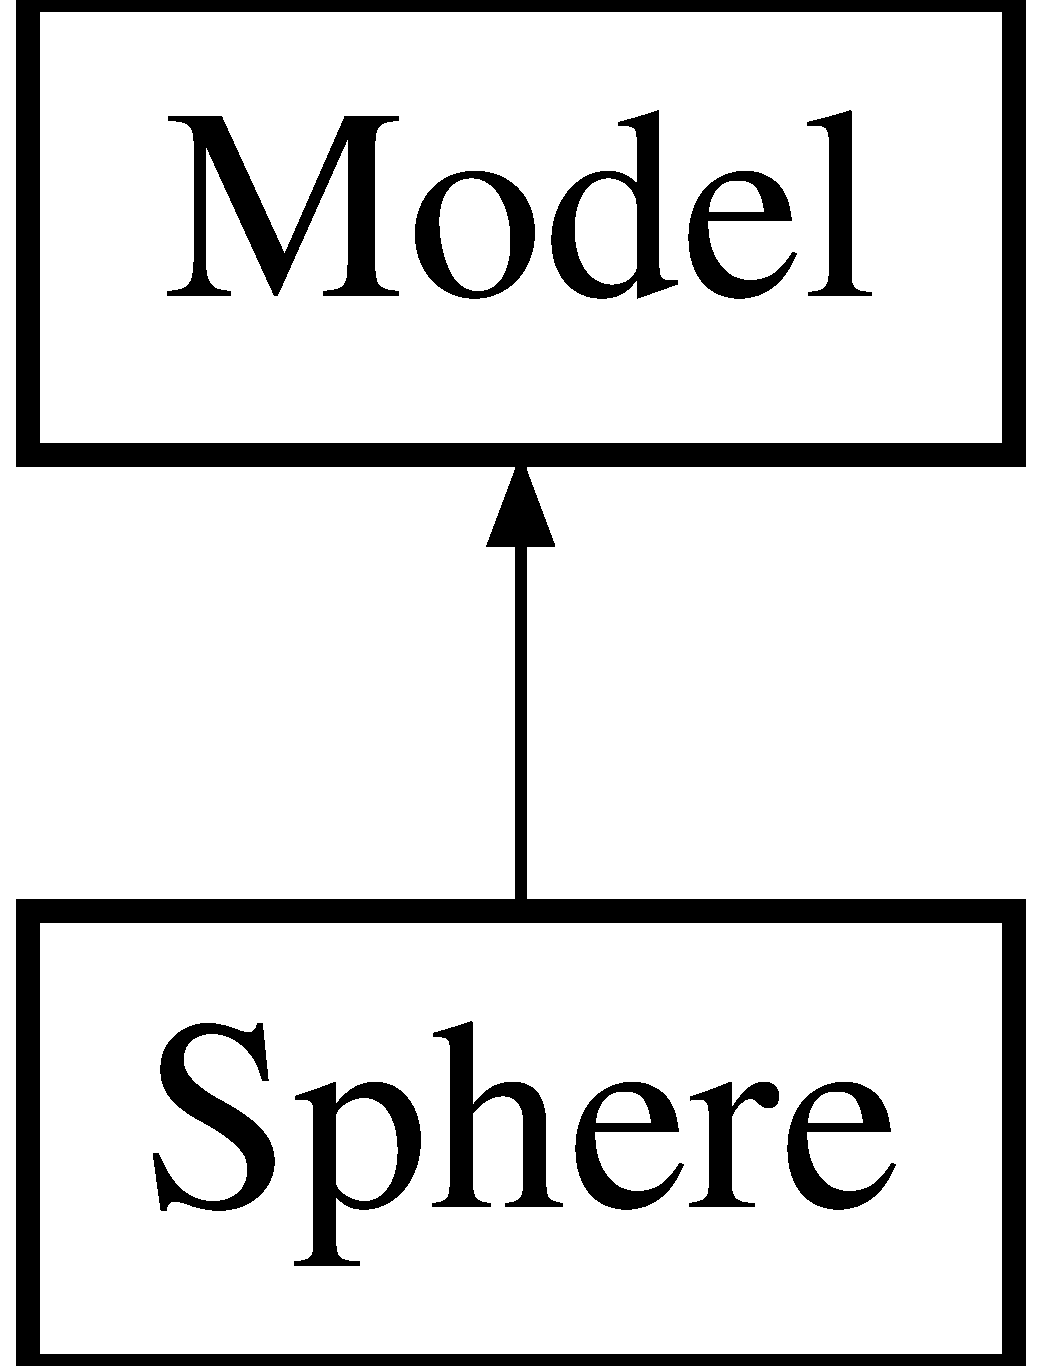
\includegraphics[height=2.000000cm]{classModel}
\end{center}
\end{figure}
\subsection*{Public Member Functions}
\begin{DoxyCompactItemize}
\item 
Eigen\+::\+Matrix$<$ G\+Lfloat, 4, 4 $>$ \hyperlink{classModel_af37e550b25274838de666ddc7e2167d6}{Get\+Model\+Matrix} ()
\item 
void \hyperlink{classModel_a6b79c9e0c9abc50896e70fe1fabff4e7}{Set\+Model\+Matrix} (Eigen\+::\+Matrix$<$ G\+Lfloat, 4, 4 $>$ model)
\item 
\hyperlink{classMesh}{Mesh} \hyperlink{classModel_a332f5a4ecf9bca582e583b3ff7784bf5}{Get\+Mesh} ()
\end{DoxyCompactItemize}
\subsection*{Protected Member Functions}
\begin{DoxyCompactItemize}
\item 
\hyperlink{classModel_ae3b375de5f6df4faf74a95d64748e048}{Model} ()
\end{DoxyCompactItemize}
\subsection*{Protected Attributes}
\begin{DoxyCompactItemize}
\item 
\hyperlink{classMesh}{Mesh} \hyperlink{classModel_afe425f579d17b798e6c454a5c5e2d952}{m\+\_\+mesh}
\item 
Eigen\+::\+Matrix$<$ G\+Lfloat, 4, 4 $>$ \hyperlink{classModel_a41d60873613f3b75c8242df3bbb44ca9}{m\+\_\+model\+\_\+matrix}
\end{DoxyCompactItemize}


\subsection{Detailed Description}
Defines a model used for rendering. 

\hyperlink{classModel}{Model} is the base class for all entities that are rendered in a scene. It stores properites such as the mesh, material properties, textures, etc. It also holds the {\bfseries model matrix} which handles transforming the mesh from local coordinates to world coordinates. See \href{https://learnopengl.com/#!Getting-started/Coordinate-Systems}{\tt Here} for more details. 

\subsection{Constructor \& Destructor Documentation}
\mbox{\Hypertarget{classModel_ae3b375de5f6df4faf74a95d64748e048}\label{classModel_ae3b375de5f6df4faf74a95d64748e048}} 
\index{Model@{Model}!Model@{Model}}
\index{Model@{Model}!Model@{Model}}
\subsubsection{\texorpdfstring{Model()}{Model()}}
{\footnotesize\ttfamily Model\+::\+Model (\begin{DoxyParamCaption}{ }\end{DoxyParamCaption})\hspace{0.3cm}{\ttfamily [protected]}}

Builds a \hyperlink{classModel}{Model} with an empty mesh and identity model matrix 

\subsection{Member Function Documentation}
\mbox{\Hypertarget{classModel_a332f5a4ecf9bca582e583b3ff7784bf5}\label{classModel_a332f5a4ecf9bca582e583b3ff7784bf5}} 
\index{Model@{Model}!Get\+Mesh@{Get\+Mesh}}
\index{Get\+Mesh@{Get\+Mesh}!Model@{Model}}
\subsubsection{\texorpdfstring{Get\+Mesh()}{GetMesh()}}
{\footnotesize\ttfamily \hyperlink{classMesh}{Mesh} Model\+::\+Get\+Mesh (\begin{DoxyParamCaption}{ }\end{DoxyParamCaption})}

\begin{DoxyReturn}{Returns}
Copy of the mesh used by this model 
\end{DoxyReturn}
\mbox{\Hypertarget{classModel_af37e550b25274838de666ddc7e2167d6}\label{classModel_af37e550b25274838de666ddc7e2167d6}} 
\index{Model@{Model}!Get\+Model\+Matrix@{Get\+Model\+Matrix}}
\index{Get\+Model\+Matrix@{Get\+Model\+Matrix}!Model@{Model}}
\subsubsection{\texorpdfstring{Get\+Model\+Matrix()}{GetModelMatrix()}}
{\footnotesize\ttfamily Eigen\+::\+Matrix$<$ G\+Lfloat, 4, 4 $>$ Model\+::\+Get\+Model\+Matrix (\begin{DoxyParamCaption}{ }\end{DoxyParamCaption})}

\begin{DoxyReturn}{Returns}
The model matrix 
\end{DoxyReturn}
\mbox{\Hypertarget{classModel_a6b79c9e0c9abc50896e70fe1fabff4e7}\label{classModel_a6b79c9e0c9abc50896e70fe1fabff4e7}} 
\index{Model@{Model}!Set\+Model\+Matrix@{Set\+Model\+Matrix}}
\index{Set\+Model\+Matrix@{Set\+Model\+Matrix}!Model@{Model}}
\subsubsection{\texorpdfstring{Set\+Model\+Matrix()}{SetModelMatrix()}}
{\footnotesize\ttfamily void Model\+::\+Set\+Model\+Matrix (\begin{DoxyParamCaption}\item[{Eigen\+::\+Matrix$<$ G\+Lfloat, 4, 4 $>$}]{model }\end{DoxyParamCaption})}

Sets the model matrix 
\begin{DoxyParams}{Parameters}
{\em model} & Matrix to be set as the model matrix \\
\hline
\end{DoxyParams}


\subsection{Member Data Documentation}
\mbox{\Hypertarget{classModel_afe425f579d17b798e6c454a5c5e2d952}\label{classModel_afe425f579d17b798e6c454a5c5e2d952}} 
\index{Model@{Model}!m\+\_\+mesh@{m\+\_\+mesh}}
\index{m\+\_\+mesh@{m\+\_\+mesh}!Model@{Model}}
\subsubsection{\texorpdfstring{m\+\_\+mesh}{m\_mesh}}
{\footnotesize\ttfamily \hyperlink{classMesh}{Mesh} Model\+::m\+\_\+mesh\hspace{0.3cm}{\ttfamily [protected]}}

The mesh for this model \mbox{\Hypertarget{classModel_a41d60873613f3b75c8242df3bbb44ca9}\label{classModel_a41d60873613f3b75c8242df3bbb44ca9}} 
\index{Model@{Model}!m\+\_\+model\+\_\+matrix@{m\+\_\+model\+\_\+matrix}}
\index{m\+\_\+model\+\_\+matrix@{m\+\_\+model\+\_\+matrix}!Model@{Model}}
\subsubsection{\texorpdfstring{m\+\_\+model\+\_\+matrix}{m\_model\_matrix}}
{\footnotesize\ttfamily Eigen\+::\+Matrix$<$G\+Lfloat,4,4$>$ Model\+::m\+\_\+model\+\_\+matrix\hspace{0.3cm}{\ttfamily [protected]}}

The model matrix. This handles transforming from local model coordinates to world coordinates 

The documentation for this class was generated from the following files\+:\begin{DoxyCompactItemize}
\item 
/home/adam/\+Desktop/\+Engine/include/model.\+h\item 
/home/adam/\+Desktop/\+Engine/model.\+cpp\end{DoxyCompactItemize}

\hypertarget{classPhysicsEntity}{}\section{Physics\+Entity Class Reference}
\label{classPhysicsEntity}\index{Physics\+Entity@{Physics\+Entity}}


An entity subject to the laws of physics.  




{\ttfamily \#include $<$physics\+\_\+entity.\+h$>$}

Inheritance diagram for Physics\+Entity\+:\begin{figure}[H]
\begin{center}
\leavevmode
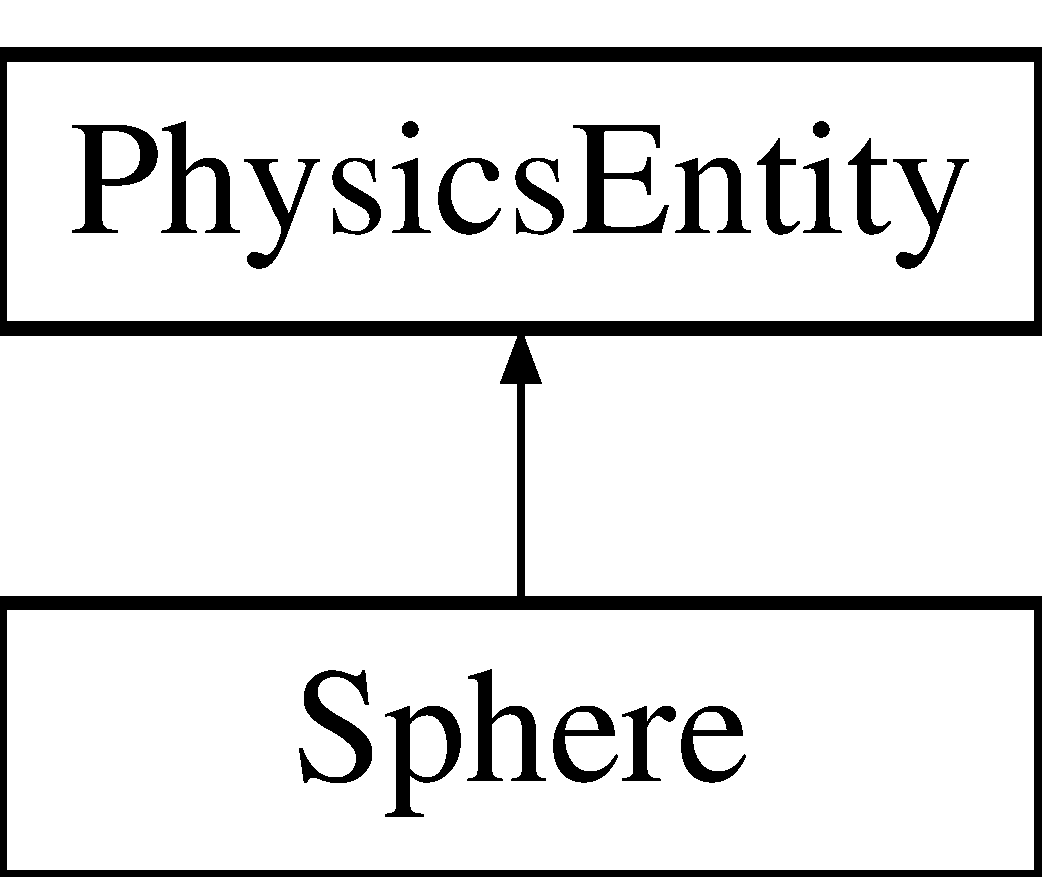
\includegraphics[height=2.000000cm]{classPhysicsEntity}
\end{center}
\end{figure}
\subsection*{Public Types}
\begin{DoxyCompactItemize}
\item 
enum \hyperlink{classPhysicsEntity_a171840d3fef1fc21c3f922b240e03538}{E\+N\+T\+I\+T\+Y\+\_\+\+T\+Y\+PE} \{ {\bfseries S\+P\+H\+E\+R\+E\+\_\+\+E\+N\+T\+I\+TY}
 \}
\end{DoxyCompactItemize}
\subsection*{Public Member Functions}
\begin{DoxyCompactItemize}
\item 
\hyperlink{classPhysicsEntity_a171840d3fef1fc21c3f922b240e03538}{E\+N\+T\+I\+T\+Y\+\_\+\+T\+Y\+PE} \hyperlink{classPhysicsEntity_a5a1eb68e1ecb2d845959addbbc915577}{Get\+Entity\+Type} ()
\item 
Vector3\+Gf \hyperlink{classPhysicsEntity_a73d263f4efb4fc87b36493f340d94a97}{Get\+Position} ()
\item 
void \hyperlink{classPhysicsEntity_a18913bb368bbe6e61e6838d7e8353bd4}{Set\+Next\+Position} (Vector3\+Gf x)
\item 
Vector3\+Gf \hyperlink{classPhysicsEntity_a2064523af6e64719996d505360e37af1}{Get\+Velocity} ()
\item 
void \hyperlink{classPhysicsEntity_a6d23d47421d535cc934405e8a7d1a43b}{Set\+Next\+Velocity} (Vector3\+Gf v)
\item 
G\+Lfloat \hyperlink{classPhysicsEntity_a07943c4b81878d402b97d1280f8c8ff9}{Get\+Mass} ()
\item 
void \hyperlink{classPhysicsEntity_a912c227d955b9a3c82e77b9732c8e5f2}{Update\+From\+Buffers} ()
\end{DoxyCompactItemize}
\subsection*{Protected Member Functions}
\begin{DoxyCompactItemize}
\item 
\hyperlink{classPhysicsEntity_a2c0cf9804f1864105849586bc91e8dea}{Physics\+Entity} ()
\end{DoxyCompactItemize}
\subsection*{Protected Attributes}
\begin{DoxyCompactItemize}
\item 
\hyperlink{classPhysicsEntity_a171840d3fef1fc21c3f922b240e03538}{E\+N\+T\+I\+T\+Y\+\_\+\+T\+Y\+PE} \hyperlink{classPhysicsEntity_a71e8887fb5fd67e84b39d99dae634daf}{m\+\_\+entity\+\_\+type}
\item 
Vector3\+Gf \hyperlink{classPhysicsEntity_afee5026bb0c5504697b7a6c4c59d8003}{m\+\_\+position}
\item 
Vector3\+Gf \hyperlink{classPhysicsEntity_abc38c58fd803d67079f25043331f0018}{m\+\_\+next\+\_\+position\+\_\+buffer}
\item 
Vector3\+Gf \hyperlink{classPhysicsEntity_ad03f63872ec7c9ddf734e92034d6e112}{m\+\_\+velocity}
\item 
Vector3\+Gf \hyperlink{classPhysicsEntity_a00034d95cc1a6f34ceaf5ad961e4afe6}{m\+\_\+next\+\_\+velocity\+\_\+buffer}
\item 
G\+Lfloat \hyperlink{classPhysicsEntity_a5a7bc5174169e169f69723d2483c2eff}{m\+\_\+mass}
\end{DoxyCompactItemize}


\subsection{Detailed Description}
An entity subject to the laws of physics. 

\hyperlink{classPhysicsEntity}{Physics\+Entity} is a base class for all objects in a scene that respond to forces and other physical phenomenon 

\subsection{Member Enumeration Documentation}
\mbox{\Hypertarget{classPhysicsEntity_a171840d3fef1fc21c3f922b240e03538}\label{classPhysicsEntity_a171840d3fef1fc21c3f922b240e03538}} 
\index{Physics\+Entity@{Physics\+Entity}!E\+N\+T\+I\+T\+Y\+\_\+\+T\+Y\+PE@{E\+N\+T\+I\+T\+Y\+\_\+\+T\+Y\+PE}}
\index{E\+N\+T\+I\+T\+Y\+\_\+\+T\+Y\+PE@{E\+N\+T\+I\+T\+Y\+\_\+\+T\+Y\+PE}!Physics\+Entity@{Physics\+Entity}}
\subsubsection{\texorpdfstring{E\+N\+T\+I\+T\+Y\+\_\+\+T\+Y\+PE}{ENTITY\_TYPE}}
{\footnotesize\ttfamily enum \hyperlink{classPhysicsEntity_a171840d3fef1fc21c3f922b240e03538}{Physics\+Entity\+::\+E\+N\+T\+I\+T\+Y\+\_\+\+T\+Y\+PE}\hspace{0.3cm}{\ttfamily [strong]}}

Enum representing the different kinds of physical entities there can be. Used in casting operations 

\subsection{Constructor \& Destructor Documentation}
\mbox{\Hypertarget{classPhysicsEntity_a2c0cf9804f1864105849586bc91e8dea}\label{classPhysicsEntity_a2c0cf9804f1864105849586bc91e8dea}} 
\index{Physics\+Entity@{Physics\+Entity}!Physics\+Entity@{Physics\+Entity}}
\index{Physics\+Entity@{Physics\+Entity}!Physics\+Entity@{Physics\+Entity}}
\subsubsection{\texorpdfstring{Physics\+Entity()}{PhysicsEntity()}}
{\footnotesize\ttfamily Physics\+Entity\+::\+Physics\+Entity (\begin{DoxyParamCaption}{ }\end{DoxyParamCaption})\hspace{0.3cm}{\ttfamily [protected]}}

Creates an instance of \hyperlink{classPhysicsEntity}{Physics\+Entity} centered at the origin, zero velocity, and unit mass 

\subsection{Member Function Documentation}
\mbox{\Hypertarget{classPhysicsEntity_a5a1eb68e1ecb2d845959addbbc915577}\label{classPhysicsEntity_a5a1eb68e1ecb2d845959addbbc915577}} 
\index{Physics\+Entity@{Physics\+Entity}!Get\+Entity\+Type@{Get\+Entity\+Type}}
\index{Get\+Entity\+Type@{Get\+Entity\+Type}!Physics\+Entity@{Physics\+Entity}}
\subsubsection{\texorpdfstring{Get\+Entity\+Type()}{GetEntityType()}}
{\footnotesize\ttfamily \hyperlink{classPhysicsEntity_a171840d3fef1fc21c3f922b240e03538}{Physics\+Entity\+::\+E\+N\+T\+I\+T\+Y\+\_\+\+T\+Y\+PE} Physics\+Entity\+::\+Get\+Entity\+Type (\begin{DoxyParamCaption}{ }\end{DoxyParamCaption})}

\begin{DoxyReturn}{Returns}
Entity type for this instance 
\end{DoxyReturn}
\mbox{\Hypertarget{classPhysicsEntity_a07943c4b81878d402b97d1280f8c8ff9}\label{classPhysicsEntity_a07943c4b81878d402b97d1280f8c8ff9}} 
\index{Physics\+Entity@{Physics\+Entity}!Get\+Mass@{Get\+Mass}}
\index{Get\+Mass@{Get\+Mass}!Physics\+Entity@{Physics\+Entity}}
\subsubsection{\texorpdfstring{Get\+Mass()}{GetMass()}}
{\footnotesize\ttfamily G\+Lfloat Physics\+Entity\+::\+Get\+Mass (\begin{DoxyParamCaption}{ }\end{DoxyParamCaption})}

\begin{DoxyReturn}{Returns}
Mass of this entity 
\end{DoxyReturn}
\mbox{\Hypertarget{classPhysicsEntity_a73d263f4efb4fc87b36493f340d94a97}\label{classPhysicsEntity_a73d263f4efb4fc87b36493f340d94a97}} 
\index{Physics\+Entity@{Physics\+Entity}!Get\+Position@{Get\+Position}}
\index{Get\+Position@{Get\+Position}!Physics\+Entity@{Physics\+Entity}}
\subsubsection{\texorpdfstring{Get\+Position()}{GetPosition()}}
{\footnotesize\ttfamily Vector3\+Gf Physics\+Entity\+::\+Get\+Position (\begin{DoxyParamCaption}{ }\end{DoxyParamCaption})}

\begin{DoxyReturn}{Returns}
Spatial position for this entity 
\end{DoxyReturn}
\mbox{\Hypertarget{classPhysicsEntity_a2064523af6e64719996d505360e37af1}\label{classPhysicsEntity_a2064523af6e64719996d505360e37af1}} 
\index{Physics\+Entity@{Physics\+Entity}!Get\+Velocity@{Get\+Velocity}}
\index{Get\+Velocity@{Get\+Velocity}!Physics\+Entity@{Physics\+Entity}}
\subsubsection{\texorpdfstring{Get\+Velocity()}{GetVelocity()}}
{\footnotesize\ttfamily Vector3\+Gf Physics\+Entity\+::\+Get\+Velocity (\begin{DoxyParamCaption}{ }\end{DoxyParamCaption})}

\begin{DoxyReturn}{Returns}
Spatial velocity for this entity 
\end{DoxyReturn}
\mbox{\Hypertarget{classPhysicsEntity_a18913bb368bbe6e61e6838d7e8353bd4}\label{classPhysicsEntity_a18913bb368bbe6e61e6838d7e8353bd4}} 
\index{Physics\+Entity@{Physics\+Entity}!Set\+Next\+Position@{Set\+Next\+Position}}
\index{Set\+Next\+Position@{Set\+Next\+Position}!Physics\+Entity@{Physics\+Entity}}
\subsubsection{\texorpdfstring{Set\+Next\+Position()}{SetNextPosition()}}
{\footnotesize\ttfamily void Physics\+Entity\+::\+Set\+Next\+Position (\begin{DoxyParamCaption}\item[{Vector3\+Gf}]{x }\end{DoxyParamCaption})}

Sets the next position buffer for this entity. This {\bfseries D\+O\+ES N\+OT} update the position until \hyperlink{classPhysicsEntity_a912c227d955b9a3c82e77b9732c8e5f2}{Update\+From\+Buffers()} is called. 
\begin{DoxyParams}{Parameters}
{\em x} & Next position for this entity \\
\hline
\end{DoxyParams}
\mbox{\Hypertarget{classPhysicsEntity_a6d23d47421d535cc934405e8a7d1a43b}\label{classPhysicsEntity_a6d23d47421d535cc934405e8a7d1a43b}} 
\index{Physics\+Entity@{Physics\+Entity}!Set\+Next\+Velocity@{Set\+Next\+Velocity}}
\index{Set\+Next\+Velocity@{Set\+Next\+Velocity}!Physics\+Entity@{Physics\+Entity}}
\subsubsection{\texorpdfstring{Set\+Next\+Velocity()}{SetNextVelocity()}}
{\footnotesize\ttfamily void Physics\+Entity\+::\+Set\+Next\+Velocity (\begin{DoxyParamCaption}\item[{Vector3\+Gf}]{v }\end{DoxyParamCaption})}

Sets the next velocity buffer for the entity. This {\bfseries D\+O\+ES N\+OT} update the velocity until \hyperlink{classPhysicsEntity_a912c227d955b9a3c82e77b9732c8e5f2}{Update\+From\+Buffers()} is called. 
\begin{DoxyParams}{Parameters}
{\em v} & Next velocity for this entity \\
\hline
\end{DoxyParams}
\mbox{\Hypertarget{classPhysicsEntity_a912c227d955b9a3c82e77b9732c8e5f2}\label{classPhysicsEntity_a912c227d955b9a3c82e77b9732c8e5f2}} 
\index{Physics\+Entity@{Physics\+Entity}!Update\+From\+Buffers@{Update\+From\+Buffers}}
\index{Update\+From\+Buffers@{Update\+From\+Buffers}!Physics\+Entity@{Physics\+Entity}}
\subsubsection{\texorpdfstring{Update\+From\+Buffers()}{UpdateFromBuffers()}}
{\footnotesize\ttfamily void Physics\+Entity\+::\+Update\+From\+Buffers (\begin{DoxyParamCaption}{ }\end{DoxyParamCaption})}

Updates internal state from buffers. This will load the next position and velocity from their corresponding buffers 

\subsection{Member Data Documentation}
\mbox{\Hypertarget{classPhysicsEntity_a71e8887fb5fd67e84b39d99dae634daf}\label{classPhysicsEntity_a71e8887fb5fd67e84b39d99dae634daf}} 
\index{Physics\+Entity@{Physics\+Entity}!m\+\_\+entity\+\_\+type@{m\+\_\+entity\+\_\+type}}
\index{m\+\_\+entity\+\_\+type@{m\+\_\+entity\+\_\+type}!Physics\+Entity@{Physics\+Entity}}
\subsubsection{\texorpdfstring{m\+\_\+entity\+\_\+type}{m\_entity\_type}}
{\footnotesize\ttfamily \hyperlink{classPhysicsEntity_a171840d3fef1fc21c3f922b240e03538}{E\+N\+T\+I\+T\+Y\+\_\+\+T\+Y\+PE} Physics\+Entity\+::m\+\_\+entity\+\_\+type\hspace{0.3cm}{\ttfamily [protected]}}

The type of this entity. Ex.) S\+P\+H\+E\+R\+E\+\_\+\+E\+N\+T\+I\+TY \mbox{\Hypertarget{classPhysicsEntity_a5a7bc5174169e169f69723d2483c2eff}\label{classPhysicsEntity_a5a7bc5174169e169f69723d2483c2eff}} 
\index{Physics\+Entity@{Physics\+Entity}!m\+\_\+mass@{m\+\_\+mass}}
\index{m\+\_\+mass@{m\+\_\+mass}!Physics\+Entity@{Physics\+Entity}}
\subsubsection{\texorpdfstring{m\+\_\+mass}{m\_mass}}
{\footnotesize\ttfamily G\+Lfloat Physics\+Entity\+::m\+\_\+mass\hspace{0.3cm}{\ttfamily [protected]}}

The mass of this entity \mbox{\Hypertarget{classPhysicsEntity_abc38c58fd803d67079f25043331f0018}\label{classPhysicsEntity_abc38c58fd803d67079f25043331f0018}} 
\index{Physics\+Entity@{Physics\+Entity}!m\+\_\+next\+\_\+position\+\_\+buffer@{m\+\_\+next\+\_\+position\+\_\+buffer}}
\index{m\+\_\+next\+\_\+position\+\_\+buffer@{m\+\_\+next\+\_\+position\+\_\+buffer}!Physics\+Entity@{Physics\+Entity}}
\subsubsection{\texorpdfstring{m\+\_\+next\+\_\+position\+\_\+buffer}{m\_next\_position\_buffer}}
{\footnotesize\ttfamily Vector3\+Gf Physics\+Entity\+::m\+\_\+next\+\_\+position\+\_\+buffer\hspace{0.3cm}{\ttfamily [protected]}}

The next predicted position of this entity. \mbox{\Hypertarget{classPhysicsEntity_a00034d95cc1a6f34ceaf5ad961e4afe6}\label{classPhysicsEntity_a00034d95cc1a6f34ceaf5ad961e4afe6}} 
\index{Physics\+Entity@{Physics\+Entity}!m\+\_\+next\+\_\+velocity\+\_\+buffer@{m\+\_\+next\+\_\+velocity\+\_\+buffer}}
\index{m\+\_\+next\+\_\+velocity\+\_\+buffer@{m\+\_\+next\+\_\+velocity\+\_\+buffer}!Physics\+Entity@{Physics\+Entity}}
\subsubsection{\texorpdfstring{m\+\_\+next\+\_\+velocity\+\_\+buffer}{m\_next\_velocity\_buffer}}
{\footnotesize\ttfamily Vector3\+Gf Physics\+Entity\+::m\+\_\+next\+\_\+velocity\+\_\+buffer\hspace{0.3cm}{\ttfamily [protected]}}

The next predicted velocity of this entity \mbox{\Hypertarget{classPhysicsEntity_afee5026bb0c5504697b7a6c4c59d8003}\label{classPhysicsEntity_afee5026bb0c5504697b7a6c4c59d8003}} 
\index{Physics\+Entity@{Physics\+Entity}!m\+\_\+position@{m\+\_\+position}}
\index{m\+\_\+position@{m\+\_\+position}!Physics\+Entity@{Physics\+Entity}}
\subsubsection{\texorpdfstring{m\+\_\+position}{m\_position}}
{\footnotesize\ttfamily Vector3\+Gf Physics\+Entity\+::m\+\_\+position\hspace{0.3cm}{\ttfamily [protected]}}

The position of this entity \mbox{\Hypertarget{classPhysicsEntity_ad03f63872ec7c9ddf734e92034d6e112}\label{classPhysicsEntity_ad03f63872ec7c9ddf734e92034d6e112}} 
\index{Physics\+Entity@{Physics\+Entity}!m\+\_\+velocity@{m\+\_\+velocity}}
\index{m\+\_\+velocity@{m\+\_\+velocity}!Physics\+Entity@{Physics\+Entity}}
\subsubsection{\texorpdfstring{m\+\_\+velocity}{m\_velocity}}
{\footnotesize\ttfamily Vector3\+Gf Physics\+Entity\+::m\+\_\+velocity\hspace{0.3cm}{\ttfamily [protected]}}

The velocity of this entity 

The documentation for this class was generated from the following files\+:\begin{DoxyCompactItemize}
\item 
/home/adam/\+Desktop/\+Engine/include/physics\+\_\+entity.\+h\item 
/home/adam/\+Desktop/\+Engine/physics\+\_\+entity.\+cpp\end{DoxyCompactItemize}

\hypertarget{classScene}{}\section{Scene Class Reference}
\label{classScene}\index{Scene@{Scene}}


A scene in the engine.  




{\ttfamily \#include $<$scene.\+h$>$}

\subsection*{Public Member Functions}
\begin{DoxyCompactItemize}
\item 
\hyperlink{classScene_ad10176d75a9cc0da56626f682d083507}{Scene} ()
\item 
\hyperlink{classScene_a0a3d0bcafa5f18639e2af91c4c43115b}{Scene} (std\+::shared\+\_\+ptr$<$ \hyperlink{classTimeIntegrator}{Time\+Integrator} $>$ integrator, \hyperlink{classConstantForceGenerator}{Constant\+Force\+Generator} cfg)
\item 
void \hyperlink{classScene_a18477e2b5b504b46f3e7d37908abb98d}{Add\+Physics\+Entity} (std\+::shared\+\_\+ptr$<$ \hyperlink{classPhysicsEntity}{Physics\+Entity} $>$ entity\+\_\+ptr)
\item 
void \hyperlink{classScene_ac20558c7452d933ce3ebe8caa1514702}{Get\+Physics\+Entity} (const G\+Luint index, std\+::shared\+\_\+ptr$<$ \hyperlink{classPhysicsEntity}{Physics\+Entity} $>$ \&entity\+\_\+ptr)
\item 
void \hyperlink{classScene_a5419dc941ee6efc29cd5cef8e7d6d414}{Add\+Model} (std\+::shared\+\_\+ptr$<$ \hyperlink{classModel}{Model} $>$ model\+\_\+ptr)
\item 
void \hyperlink{classScene_a031dc667e4152e4bfd2a8930d31320a4}{Get\+Model} (const G\+Luint index, std\+::shared\+\_\+ptr$<$ \hyperlink{classModel}{Model} $>$ \&model\+\_\+ptr, G\+Luint \&V\+AO)
\item 
G\+Luint \hyperlink{classScene_a2cadf8fe478a7e3a270902a0536751a9}{Get\+Physics\+Entity\+Count} ()
\item 
G\+Luint \hyperlink{classScene_a406df661eb7be589964dafe76f7f09c8}{Get\+Model\+Count} ()
\item 
void \hyperlink{classScene_a5fe443641612290ba78931132d1fddb5}{Step\+Physics} ()
\item 
void \hyperlink{classScene_a7edc9fabe7ef61a426cd6278a0b209fe}{Render} (\hyperlink{classShader}{Shader} shader)
\item 
void \hyperlink{classScene_a830078c354d5df8ef9b811dac7b2c7dd}{Clean\+Up} ()
\end{DoxyCompactItemize}


\subsection{Detailed Description}
A scene in the engine. 

A scene contains (pointers to) a number of \hyperlink{classPhysicsEntity}{Physics\+Entity} objects to simululate and a number of \hyperlink{classModel}{Model} objects to render. 

\subsection{Constructor \& Destructor Documentation}
\mbox{\Hypertarget{classScene_ad10176d75a9cc0da56626f682d083507}\label{classScene_ad10176d75a9cc0da56626f682d083507}} 
\index{Scene@{Scene}!Scene@{Scene}}
\index{Scene@{Scene}!Scene@{Scene}}
\subsubsection{\texorpdfstring{Scene()}{Scene()}\hspace{0.1cm}{\footnotesize\ttfamily [1/2]}}
{\footnotesize\ttfamily Scene\+::\+Scene (\begin{DoxyParamCaption}{ }\end{DoxyParamCaption})}

Creates a \hyperlink{classScene}{Scene} instance with default values for its \hyperlink{classTimeIntegrator}{Time\+Integrator} and \hyperlink{classForceGenerator}{Force\+Generator} members \mbox{\Hypertarget{classScene_a0a3d0bcafa5f18639e2af91c4c43115b}\label{classScene_a0a3d0bcafa5f18639e2af91c4c43115b}} 
\index{Scene@{Scene}!Scene@{Scene}}
\index{Scene@{Scene}!Scene@{Scene}}
\subsubsection{\texorpdfstring{Scene()}{Scene()}\hspace{0.1cm}{\footnotesize\ttfamily [2/2]}}
{\footnotesize\ttfamily Scene\+::\+Scene (\begin{DoxyParamCaption}\item[{std\+::shared\+\_\+ptr$<$ \hyperlink{classTimeIntegrator}{Time\+Integrator} $>$}]{integrator,  }\item[{\hyperlink{classConstantForceGenerator}{Constant\+Force\+Generator}}]{cfg }\end{DoxyParamCaption})}

Creates a \hyperlink{classScene}{Scene} instance with the provided \hyperlink{classTimeIntegrator}{Time\+Integrator} and \hyperlink{classForceGenerator}{Force\+Generator} members 
\begin{DoxyParams}{Parameters}
{\em integrator} & Time\+Ingrator instance to handle time evolution of the Physics\+Entities in the scene \\
\hline
{\em cfg} & \hyperlink{classConstantForceGenerator}{Constant\+Force\+Generator} used to generate a spatially and temporally uniform force \\
\hline
\end{DoxyParams}


\subsection{Member Function Documentation}
\mbox{\Hypertarget{classScene_a5419dc941ee6efc29cd5cef8e7d6d414}\label{classScene_a5419dc941ee6efc29cd5cef8e7d6d414}} 
\index{Scene@{Scene}!Add\+Model@{Add\+Model}}
\index{Add\+Model@{Add\+Model}!Scene@{Scene}}
\subsubsection{\texorpdfstring{Add\+Model()}{AddModel()}}
{\footnotesize\ttfamily void Scene\+::\+Add\+Model (\begin{DoxyParamCaption}\item[{std\+::shared\+\_\+ptr$<$ \hyperlink{classModel}{Model} $>$}]{model\+\_\+ptr }\end{DoxyParamCaption})}

Adds a \hyperlink{classModel}{Model} to the scene 
\begin{DoxyParams}{Parameters}
{\em model\+\_\+ptr} & a shared pointer to the model to be added to the scene \\
\hline
\end{DoxyParams}
\mbox{\Hypertarget{classScene_a18477e2b5b504b46f3e7d37908abb98d}\label{classScene_a18477e2b5b504b46f3e7d37908abb98d}} 
\index{Scene@{Scene}!Add\+Physics\+Entity@{Add\+Physics\+Entity}}
\index{Add\+Physics\+Entity@{Add\+Physics\+Entity}!Scene@{Scene}}
\subsubsection{\texorpdfstring{Add\+Physics\+Entity()}{AddPhysicsEntity()}}
{\footnotesize\ttfamily void Scene\+::\+Add\+Physics\+Entity (\begin{DoxyParamCaption}\item[{std\+::shared\+\_\+ptr$<$ \hyperlink{classPhysicsEntity}{Physics\+Entity} $>$}]{entity\+\_\+ptr }\end{DoxyParamCaption})}

Add a \hyperlink{classPhysicsEntity}{Physics\+Entity} to the \hyperlink{classScene}{Scene}. 
\begin{DoxyParams}{Parameters}
{\em entity\+\_\+ptr} & a shared pointer to the \hyperlink{classPhysicsEntity}{Physics\+Entity} to be added to the scene \\
\hline
\end{DoxyParams}
\mbox{\Hypertarget{classScene_a830078c354d5df8ef9b811dac7b2c7dd}\label{classScene_a830078c354d5df8ef9b811dac7b2c7dd}} 
\index{Scene@{Scene}!Clean\+Up@{Clean\+Up}}
\index{Clean\+Up@{Clean\+Up}!Scene@{Scene}}
\subsubsection{\texorpdfstring{Clean\+Up()}{CleanUp()}}
{\footnotesize\ttfamily void Scene\+::\+Clean\+Up (\begin{DoxyParamCaption}{ }\end{DoxyParamCaption})}

Removes all \hyperlink{classModel}{Model} data from the G\+PU \mbox{\Hypertarget{classScene_a031dc667e4152e4bfd2a8930d31320a4}\label{classScene_a031dc667e4152e4bfd2a8930d31320a4}} 
\index{Scene@{Scene}!Get\+Model@{Get\+Model}}
\index{Get\+Model@{Get\+Model}!Scene@{Scene}}
\subsubsection{\texorpdfstring{Get\+Model()}{GetModel()}}
{\footnotesize\ttfamily void Scene\+::\+Get\+Model (\begin{DoxyParamCaption}\item[{const G\+Luint}]{index,  }\item[{std\+::shared\+\_\+ptr$<$ \hyperlink{classModel}{Model} $>$ \&}]{model\+\_\+ptr,  }\item[{G\+Luint \&}]{V\+AO }\end{DoxyParamCaption})}

Loads the \hyperlink{classModel}{Model} at the given index into the supplied shared pointer 
\begin{DoxyParams}{Parameters}
{\em index} & index into the \hyperlink{classModel}{Model} list for this \hyperlink{classScene}{Scene} \\
\hline
{\em model\+\_\+ptr} & pointer that will be modifed to point to the \hyperlink{classModel}{Model} at the given index \\
\hline
{\em V\+AO} & uint that will be modifed to store the vertex array object id for the \hyperlink{classModel}{Model} \\
\hline
\end{DoxyParams}
\mbox{\Hypertarget{classScene_a406df661eb7be589964dafe76f7f09c8}\label{classScene_a406df661eb7be589964dafe76f7f09c8}} 
\index{Scene@{Scene}!Get\+Model\+Count@{Get\+Model\+Count}}
\index{Get\+Model\+Count@{Get\+Model\+Count}!Scene@{Scene}}
\subsubsection{\texorpdfstring{Get\+Model\+Count()}{GetModelCount()}}
{\footnotesize\ttfamily G\+Luint Scene\+::\+Get\+Model\+Count (\begin{DoxyParamCaption}{ }\end{DoxyParamCaption})}

\begin{DoxyReturn}{Returns}
The number of Models in the \hyperlink{classScene}{Scene} 
\end{DoxyReturn}
\mbox{\Hypertarget{classScene_ac20558c7452d933ce3ebe8caa1514702}\label{classScene_ac20558c7452d933ce3ebe8caa1514702}} 
\index{Scene@{Scene}!Get\+Physics\+Entity@{Get\+Physics\+Entity}}
\index{Get\+Physics\+Entity@{Get\+Physics\+Entity}!Scene@{Scene}}
\subsubsection{\texorpdfstring{Get\+Physics\+Entity()}{GetPhysicsEntity()}}
{\footnotesize\ttfamily void Scene\+::\+Get\+Physics\+Entity (\begin{DoxyParamCaption}\item[{const G\+Luint}]{index,  }\item[{std\+::shared\+\_\+ptr$<$ \hyperlink{classPhysicsEntity}{Physics\+Entity} $>$ \&}]{entity\+\_\+ptr }\end{DoxyParamCaption})}

Loads the \hyperlink{classPhysicsEntity}{Physics\+Entity} at the given index into the supplied shared pointer 
\begin{DoxyParams}{Parameters}
{\em index} & index into the \hyperlink{classPhysicsEntity}{Physics\+Entity} list for this \hyperlink{classScene}{Scene} \\
\hline
{\em entity\+\_\+ptr} & pointer that will be modified to point to the \hyperlink{classPhysicsEntity}{Physics\+Entity} at the given index \\
\hline
\end{DoxyParams}
\mbox{\Hypertarget{classScene_a2cadf8fe478a7e3a270902a0536751a9}\label{classScene_a2cadf8fe478a7e3a270902a0536751a9}} 
\index{Scene@{Scene}!Get\+Physics\+Entity\+Count@{Get\+Physics\+Entity\+Count}}
\index{Get\+Physics\+Entity\+Count@{Get\+Physics\+Entity\+Count}!Scene@{Scene}}
\subsubsection{\texorpdfstring{Get\+Physics\+Entity\+Count()}{GetPhysicsEntityCount()}}
{\footnotesize\ttfamily G\+Luint Scene\+::\+Get\+Physics\+Entity\+Count (\begin{DoxyParamCaption}{ }\end{DoxyParamCaption})}

\begin{DoxyReturn}{Returns}
The number of Physics Entites in the \hyperlink{classScene}{Scene} 
\end{DoxyReturn}
\mbox{\Hypertarget{classScene_a7edc9fabe7ef61a426cd6278a0b209fe}\label{classScene_a7edc9fabe7ef61a426cd6278a0b209fe}} 
\index{Scene@{Scene}!Render@{Render}}
\index{Render@{Render}!Scene@{Scene}}
\subsubsection{\texorpdfstring{Render()}{Render()}}
{\footnotesize\ttfamily void Scene\+::\+Render (\begin{DoxyParamCaption}\item[{\hyperlink{classShader}{Shader}}]{shader }\end{DoxyParamCaption})}

Renders the Models in the \hyperlink{classScene}{Scene} to the screen \mbox{\Hypertarget{classScene_a5fe443641612290ba78931132d1fddb5}\label{classScene_a5fe443641612290ba78931132d1fddb5}} 
\index{Scene@{Scene}!Step\+Physics@{Step\+Physics}}
\index{Step\+Physics@{Step\+Physics}!Scene@{Scene}}
\subsubsection{\texorpdfstring{Step\+Physics()}{StepPhysics()}}
{\footnotesize\ttfamily void Scene\+::\+Step\+Physics (\begin{DoxyParamCaption}{ }\end{DoxyParamCaption})}

Moves the physical simulation one time step forward 

The documentation for this class was generated from the following files\+:\begin{DoxyCompactItemize}
\item 
/home/adam/\+Desktop/\+Engine/include/scene.\+h\item 
/home/adam/\+Desktop/\+Engine/scene.\+cpp\end{DoxyCompactItemize}

\hypertarget{classShader}{}\section{Shader Class Reference}
\label{classShader}\index{Shader@{Shader}}
\subsection*{Public Member Functions}
\begin{DoxyCompactItemize}
\item 
\mbox{\Hypertarget{classShader_a03421a8419cdad4b84cf58ecdb156879}\label{classShader_a03421a8419cdad4b84cf58ecdb156879}} 
{\bfseries Shader} (const G\+Lchar $\ast$vertex\+Path, const G\+Lchar $\ast$fragment\+Path)
\item 
\mbox{\Hypertarget{classShader_a6b11327cff651ffdb22988b6917b1650}\label{classShader_a6b11327cff651ffdb22988b6917b1650}} 
void {\bfseries Use} ()
\end{DoxyCompactItemize}
\subsection*{Public Attributes}
\begin{DoxyCompactItemize}
\item 
\mbox{\Hypertarget{classShader_a51b23253846bc84dcc2ef06612679012}\label{classShader_a51b23253846bc84dcc2ef06612679012}} 
G\+Luint {\bfseries Program}
\end{DoxyCompactItemize}


The documentation for this class was generated from the following files\+:\begin{DoxyCompactItemize}
\item 
/home/adam/\+Desktop/\+Engine/include/shader.\+h\item 
/home/adam/\+Desktop/\+Engine/shader.\+cpp\end{DoxyCompactItemize}

\hypertarget{classSphere}{}\section{Sphere Class Reference}
\label{classSphere}\index{Sphere@{Sphere}}


A sphere.  




{\ttfamily \#include $<$sphere.\+h$>$}

Inheritance diagram for Sphere\+:\begin{figure}[H]
\begin{center}
\leavevmode
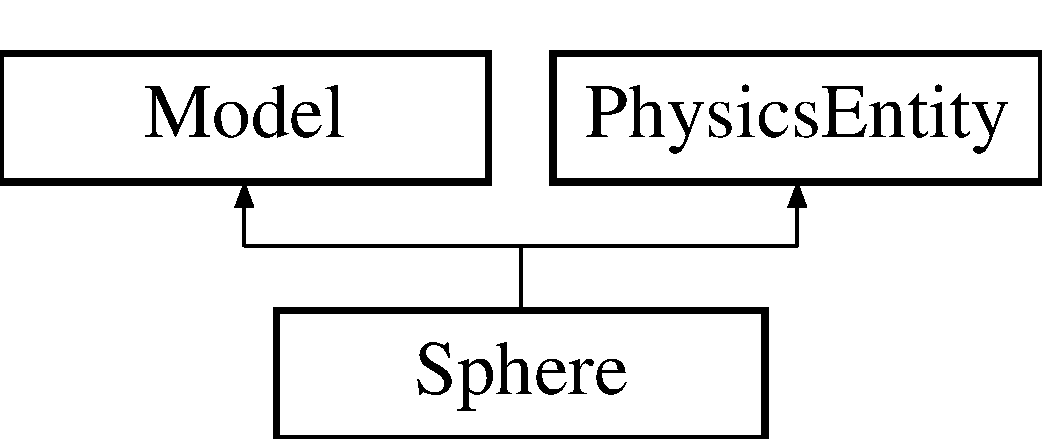
\includegraphics[height=2.000000cm]{classSphere}
\end{center}
\end{figure}
\subsection*{Public Member Functions}
\begin{DoxyCompactItemize}
\item 
\hyperlink{classSphere_a890a63ff583cb88e7ec4e840b4ef5eb9}{Sphere} ()
\item 
\hyperlink{classSphere_a6d47af660fd83089c6b26519e3d1ba0b}{Sphere} (G\+Lfloat radius, Vector3\+Gf position, Vector3\+Gf velocity, G\+Lfloat mass)
\item 
void \hyperlink{classSphere_acc0ef3890c5c5aa2758c347219e55801}{Update\+From\+Buffers} ()
\end{DoxyCompactItemize}
\subsection*{Additional Inherited Members}


\subsection{Detailed Description}
A sphere. 

A \hyperlink{classSphere}{Sphere} is defined by a center and a radius. \hyperlink{classSphere}{Sphere} extends both \hyperlink{classModel}{Model} and \hyperlink{classPhysicsEntity}{Physics\+Entity}. As such is will be rendered to the screen and act under the influence of forces 

\subsection{Constructor \& Destructor Documentation}
\mbox{\Hypertarget{classSphere_a890a63ff583cb88e7ec4e840b4ef5eb9}\label{classSphere_a890a63ff583cb88e7ec4e840b4ef5eb9}} 
\index{Sphere@{Sphere}!Sphere@{Sphere}}
\index{Sphere@{Sphere}!Sphere@{Sphere}}
\subsubsection{\texorpdfstring{Sphere()}{Sphere()}\hspace{0.1cm}{\footnotesize\ttfamily [1/2]}}
{\footnotesize\ttfamily Sphere\+::\+Sphere (\begin{DoxyParamCaption}{ }\end{DoxyParamCaption})}

Constructs a \hyperlink{classSphere}{Sphere} of radius 1.\+0, mass 1.\+0, centered at the origin \mbox{\Hypertarget{classSphere_a6d47af660fd83089c6b26519e3d1ba0b}\label{classSphere_a6d47af660fd83089c6b26519e3d1ba0b}} 
\index{Sphere@{Sphere}!Sphere@{Sphere}}
\index{Sphere@{Sphere}!Sphere@{Sphere}}
\subsubsection{\texorpdfstring{Sphere()}{Sphere()}\hspace{0.1cm}{\footnotesize\ttfamily [2/2]}}
{\footnotesize\ttfamily Sphere\+::\+Sphere (\begin{DoxyParamCaption}\item[{G\+Lfloat}]{radius,  }\item[{Vector3\+Gf}]{position,  }\item[{Vector3\+Gf}]{velocity,  }\item[{G\+Lfloat}]{mass }\end{DoxyParamCaption})}

Constructs a sphere 
\begin{DoxyParams}{Parameters}
{\em radius} & radius of the \hyperlink{classSphere}{Sphere} \\
\hline
{\em position} & position of the \hyperlink{classSphere}{Sphere} (ie its center) \\
\hline
{\em velocity} & velocity of the \hyperlink{classSphere}{Sphere} \\
\hline
{\em mass} & mass of the \hyperlink{classSphere}{Sphere} \\
\hline
\end{DoxyParams}


\subsection{Member Function Documentation}
\mbox{\Hypertarget{classSphere_acc0ef3890c5c5aa2758c347219e55801}\label{classSphere_acc0ef3890c5c5aa2758c347219e55801}} 
\index{Sphere@{Sphere}!Update\+From\+Buffers@{Update\+From\+Buffers}}
\index{Update\+From\+Buffers@{Update\+From\+Buffers}!Sphere@{Sphere}}
\subsubsection{\texorpdfstring{Update\+From\+Buffers()}{UpdateFromBuffers()}}
{\footnotesize\ttfamily void Sphere\+::\+Update\+From\+Buffers (\begin{DoxyParamCaption}{ }\end{DoxyParamCaption})}

Loads the next position and velocity values from their respective buffers 

The documentation for this class was generated from the following files\+:\begin{DoxyCompactItemize}
\item 
/home/adam/\+Desktop/\+Engine/include/sphere.\+h\item 
/home/adam/\+Desktop/\+Engine/sphere.\+cpp\end{DoxyCompactItemize}

\hypertarget{classTimeIntegrator}{}\section{Time\+Integrator Class Reference}
\label{classTimeIntegrator}\index{Time\+Integrator@{Time\+Integrator}}


An abstact base class for all grid based numerical O\+DE solvers for Newton\textquotesingle{}s laws.  




{\ttfamily \#include $<$time\+\_\+integrator.\+h$>$}

Inheritance diagram for Time\+Integrator\+:\begin{figure}[H]
\begin{center}
\leavevmode
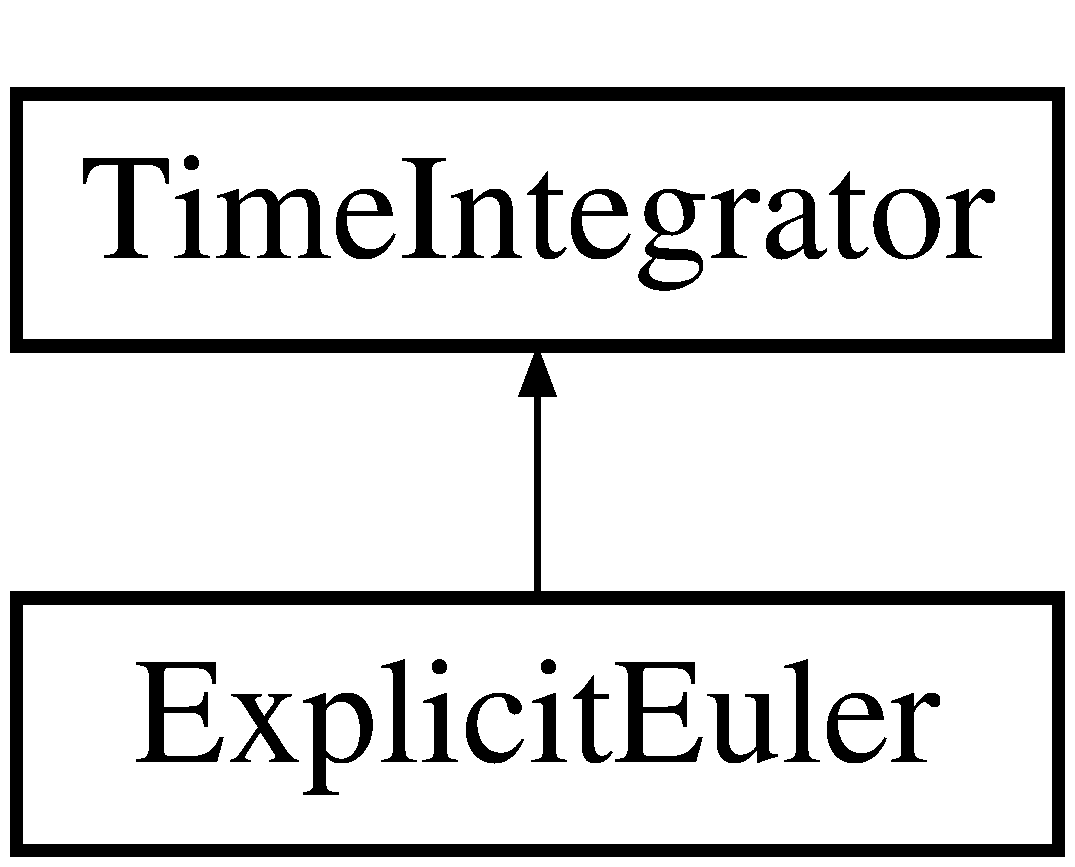
\includegraphics[height=2.000000cm]{classTimeIntegrator}
\end{center}
\end{figure}
\subsection*{Public Member Functions}
\begin{DoxyCompactItemize}
\item 
virtual void \hyperlink{classTimeIntegrator_ad69eadc41d788f355959428ff9f84608}{Solve} (const Vector3\+Gf xi, const Vector3\+Gf vi, const G\+Lfloat mass, const Vector3\+Gf F, Vector3\+Gf \&xf, Vector3\+Gf \&vf)=0
\end{DoxyCompactItemize}
\subsection*{Protected Attributes}
\begin{DoxyCompactItemize}
\item 
\mbox{\Hypertarget{classTimeIntegrator_a8912a1a1f00d49556509a91dd999991f}\label{classTimeIntegrator_a8912a1a1f00d49556509a91dd999991f}} 
G\+Lfloat {\bfseries m\+\_\+dt}
\end{DoxyCompactItemize}


\subsection{Detailed Description}
An abstact base class for all grid based numerical O\+DE solvers for Newton\textquotesingle{}s laws. 

\subsection{Member Function Documentation}
\mbox{\Hypertarget{classTimeIntegrator_ad69eadc41d788f355959428ff9f84608}\label{classTimeIntegrator_ad69eadc41d788f355959428ff9f84608}} 
\index{Time\+Integrator@{Time\+Integrator}!Solve@{Solve}}
\index{Solve@{Solve}!Time\+Integrator@{Time\+Integrator}}
\subsubsection{\texorpdfstring{Solve()}{Solve()}}
{\footnotesize\ttfamily virtual void Time\+Integrator\+::\+Solve (\begin{DoxyParamCaption}\item[{const Vector3\+Gf}]{xi,  }\item[{const Vector3\+Gf}]{vi,  }\item[{const G\+Lfloat}]{mass,  }\item[{const Vector3\+Gf}]{F,  }\item[{Vector3\+Gf \&}]{xf,  }\item[{Vector3\+Gf \&}]{vf }\end{DoxyParamCaption})\hspace{0.3cm}{\ttfamily [pure virtual]}}

Solves Newton\textquotesingle{}s equations of motion 
\begin{DoxyParams}{Parameters}
{\em xi} & initial position of entity \\
\hline
{\em vi} & initial velocity of entity \\
\hline
{\em mass} & mass of entity \\
\hline
{\em F} & force vector acting on the entity \\
\hline
{\em xf} & final position of entity. This will be updated with the new position for the next time step \\
\hline
{\em vf} & final velocity of entity. This will be updated with the new position for the next time step \\
\hline
\end{DoxyParams}


Implemented in \hyperlink{classExplicitEuler_aee3f98264fab0eac7517d9dc8487ecb4}{Explicit\+Euler}.



The documentation for this class was generated from the following file\+:\begin{DoxyCompactItemize}
\item 
/home/adam/\+Desktop/\+Engine/include/time\+\_\+integrator.\+h\end{DoxyCompactItemize}

%--- End generated contents ---

% Index
\backmatter
\newpage
\phantomsection
\clearemptydoublepage
\addcontentsline{toc}{chapter}{Index}
\printindex

\end{document}
